\PassOptionsToPackage{table,usenames,dvipsnames,x11names}{xcolor}
\documentclass[english,serif,mathserif]{beamer}
\usetheme[informal]{gc3}

\usepackage[T1]{fontenc}
\usepackage[utf8]{inputenc}
\usepackage{babel}

\usepackage{gc3}

\usepackage{colortbl}
\makeatletter
\rowcolors{1}{uzh@blue!10}{white}
\makeatother

\usepackage{dcolumn}
\newcolumntype{d}[1]{D{.}{\cdot}{#1} }


\begin{document}

%% Optional Argument in [Brackets]: Short Title for Footline
\title[Spark]{An Insufficient Introduction to Spark}
\subtitle{Part 2: RDDs and operations on them}
\author{Riccardo Murri \texttt{<riccardo.murri@gmail.com>}}
\date{2019-02-11}

%% Makes the title slide
\maketitle


\part{Spark}
\begin{frame}
  \frametitle{What is Spark?}
  \small

  \begin{center}
    {\bfseries \href{http://spark.apache.org}{Apache Spark} is a general-purpose
      \\ distributed computation framework.}
  \end{center}
  \+
  \begin{itemize}
  \item computation model based on directed acyclic graphs (DAG)
    \begin{itemize}
    \item Spark does the mapping onto Map/Reduce stages
    \item can do its own scheduling if no M/R engine available
    \end{itemize}

  \item supports interactive use:
    \begin{itemize}
    \item good for data exploration
    \end{itemize}

  \item can keep data in-memory:
    \begin{itemize}
    \item good for loop-intensive algorithms
    \end{itemize}

  \item has a rich feature-set to make programming easier \\ (in Scala, Java, Python, R)
    \begin{itemize}
    \item including ML and graph-processing libraries
    \end{itemize}

  \end{itemize}
\end{frame}


\begin{frame}
  \frametitle{Flexibility of Spark runtime}

  The spark runtime can be deployed on:
  \begin{itemize}
  \item
    a single machine (local)
  \item
    a set of pre-defined machines (stand-alone)
  \item
    a dedicated cluster (YARN/Mesos)
  \end{itemize}

  \+
  The development workflow is that you start small (local) and scale up to
  one of the other solutions, depending on your needs and resources.

  \+
  Often, you don't need to change \emph{any} code to go between these
  methods of deployment!
\end{frame}


\begin{frame}
  Recall what was hard about distributed computing:
  \begin{enumerate}
  \item
    distributing work to the available resources
  \item
    orchestrating task execution
  \item
    collecting results
  \end{enumerate}

  \+
  This is what a ``framework'' like Spark does for us.

  \+
  At its most basic, it consists of a \textbf{driver} and \textbf{workers}.
\end{frame}


\begin{frame}
  \frametitle{Spark Architecture Overview}

  \begin{center}
    A running Spark system consists of a single \textbf{driver}
    and a set of \textbf{workers}.

    \+
    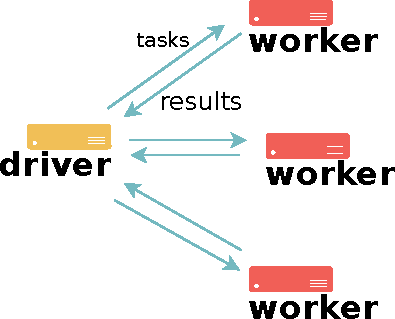
\includegraphics{fig/spark_architecture.pdf}
  \end{center}
\end{frame}


\begin{frame}
  \frametitle{Driver}

  \begin{columns}
    \begin{column}{0.5\textwidth}
      \begin{itemize}
      \item
        coordinates the work to be done
      \item
        keeps track of tasks
      \item
        communicates with the workers (and the user)
      \end{itemize}
    \end{column}
    \begin{column}{0.5\textwidth}
      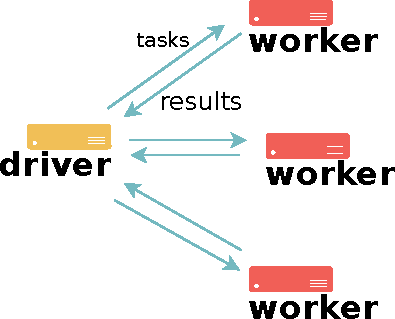
\includegraphics[height=0.45\textheight]{fig/spark_architecture.pdf}
    \end{column}
  \end{columns}
\end{frame}


\begin{frame}
  \frametitle{Workers}

  \begin{columns}
    \begin{column}{0.5\textwidth}
      \begin{itemize}
      \item
        receive tasks to be done from the driver
      \item
        store data in-memory or on disk
      \item
        perform calculations
      \item
        return results to the driver
  \end{itemize}
    \end{column}
    \begin{column}{0.5\textwidth}
      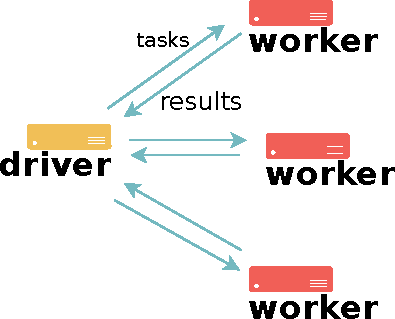
\includegraphics[height=0.45\textheight]{fig/spark_architecture.pdf}
    \end{column}
  \end{columns}
\end{frame}


\part{RDDs: basic data manipulation}
\begin{frame}
  \frametitle{Spark Context}
  \smaller

  \begin{center}
    The user's entry point to Spark is the \textbf{Spark Context} \\
    which provides an interface to generate RDDs \\ (i.e., inject data into the
    system).

    \+
    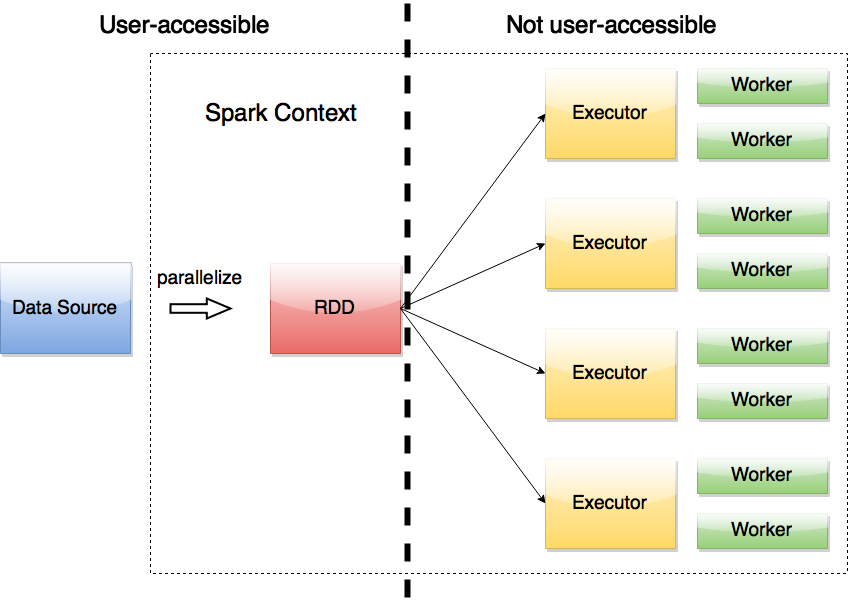
\includegraphics[width=0.80\linewidth]{fig/spark-context.png}
  \end{center}
\end{frame}


\begin{frame}[fragile]
  \frametitle{Spark Context}
  \smaller

  \begin{center}
    The user's entry point to Spark is the \textbf{Spark Context} \\
    which provides an interface to generate RDDs \\ (i.e., inject data into the
    system).

    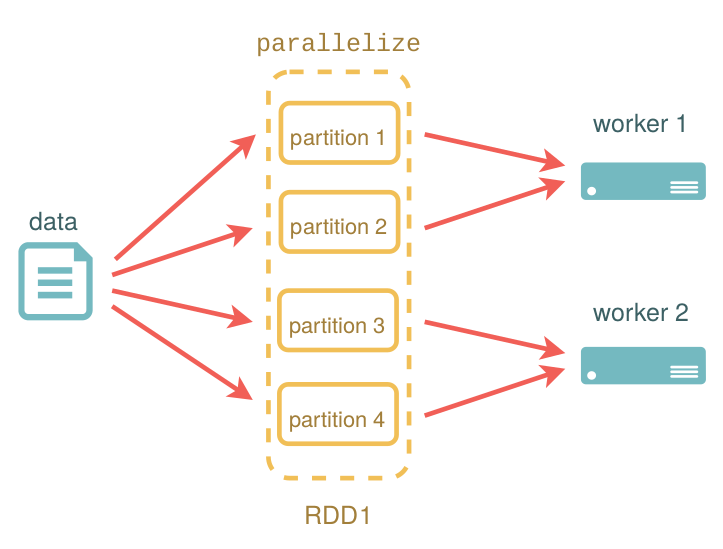
\includegraphics[width=0.75\linewidth]{fig/parallelize.png}

    \lstinline|rdd1 = sc.parallelize(data, 4)|
  \end{center}
\end{frame}


\begin{frame}[fragile]
  \frametitle{Creating RDDs}
  \begin{center}
    \begin{python}
      rdd1 = ~\HL{sc}~.parallelize(data, 4)
    \end{python}

      \+
      This is the ``Spark Context'' Python object.

      \+ It is automatically available in our Jupyter notebooks and in
      the \texttt{pyspark} shell.
    \end{center}
\end{frame}


\begin{frame}[fragile]
  \frametitle{Creating RDDs}
  \begin{center}
    \begin{python}
      rdd1 = sc.~\HL{parallelize}~(data, 4)
    \end{python}

    \+ The \texttt{.parallelize()} method is used to \emph{copy} data
    from Python into the Spark system.
  \end{center}
\end{frame}


\begin{frame}[fragile]
  \frametitle{Creating RDDs}
  \begin{center}
    \begin{python}
      rdd1 = sc.parallelize(~\HL{data}~, 4)
    \end{python}

      \+
      \emph{Any} Python sequence can be used as data.
    \end{center}
\end{frame}


\begin{frame}[fragile]
  \frametitle{Creating RDDs}
  \begin{center}
    \begin{python}
      rdd1 = sc.parallelize(data, ~\HL{4}~)
    \end{python}

    \+ This is the number of ``partitions'' to divide the data into.
    Each partition can be processed \\ \emph{independently} by a worker.

    \+ Variable \texttt{sc.defaultParallelism} holds the default
    number of executors; a good starting point for the number of
    partitions is \texttt{sc.defaultParallelism*4}
    ---~adjust up or down depending on size of the data.
    \end{center}
\end{frame}


\begin{frame}[fragile]
  \frametitle{Loading data}
  \begin{center}
    \begin{python}
rdd2 = sc.textFile('hdfs:///shakespeare.txt.gz')
    \end{python}

    \+ For \emph{actual, real} data processing you would rather
    read data from a file or another data source!
  \end{center}
\end{frame}


\begin{frame}[fragile]
  \frametitle{Loading data}
  \begin{center}
    \begin{python}
rdd2 = sc.~\HL{textFile}~('hdfs:///shakespeare.txt.gz')
    \end{python}

    \+\small There are multiple functions for loading data \\ in
    different ways:
    \begin{itemize}
    \item \texttt{sc.textFile()}: load and chunk a text file (possibly compressed)
    \item \texttt{binaryFiles()}: \texttt{wholeTextFiles()}: Read a
      directory of files. Each file is read as a single record and
      returned in a key-value pair, where the key is the path of each
      file, the value is the content of each file.
    \item \texttt{binaryRecords()}: read a binary file and chop it in
      records of the specified length.
    \end{itemize}
  \end{center}
\end{frame}


\begin{frame}[fragile]
  \frametitle{Loading data}
  \begin{center}
    \begin{python}
rdd2 = sc.textFile('~\HL{hdfs://}~/shakespeare.txt.gz')
    \end{python}

    \+ All paths can be a local filesystem path (prefix
    \texttt{file://}), a HDFS location (prefix \texttt{hdfs://}), or
    any otherfilesystem visible from the \emph{entire} Hadoop cluster.
  \end{center}
\end{frame}


\begin{frame}[fragile]
  \frametitle{Creating RDDs}
  \begin{center}
    \begin{python}
      ~\HL{rdd1}~ = sc.parallelize(data, 4)

~\HL{rdd2}~ = sc.textFile('hdfs:///shakespeare.txt.gz')
    \end{python}

      \+
      An RDD is the result of entering unstructured data into Spark.
    \end{center}
\end{frame}


\begin{frame}

  \frametitle{RDD: Resilient Distributed Dataset}

  An RDD is the primary interface of every Spark application:
  \begin{itemize}
  \item \textbf{ordered immutable collection} of arbitrary data
  \item provides an interface to the user to access and operate on the data
  \item keeps track of lineage
  \item tracks distribution of data across the workers
  \end{itemize}

  \+ \textbf{Spark applications feed data into RDDs
    and subsequently operate on them to compute the desired result.}
\end{frame}


\begin{frame}
  \frametitle{Transformations and Actions}

  Once an RDD is created, it is \textbf{immutable}.

  \+
  There are two classes of operations that can be applied to a given RDD:
  \begin{itemize}
  \item \textbf{transformations:} create a new (output) RDD by applying some operation on
    the data of the input RDD;
  \item \textbf{actions:} take data out of an RDD and into another data
    structure (e.g., list or dictionary)
  \end{itemize}
\end{frame}


\begin{frame}
  \frametitle{Actions}

  Actions take data out of an RDD and into a host language data
  structure (e.g., list or dictionary)
  \begin{itemize}
  \item converts to host language native data structures
  \item output data is collected on the \emph{driver} process: \\
    risk of a memory overflow!
  \end{itemize}
\end{frame}


\begin{frame}[fragile]
  \frametitle{Actions on all RDDs}

Actions available on \emph{all} RDDs include:
\begin{itemize}
\item
  \lstinline!collect! -- return a list of all elements of the RDD to the driver
  (often a bad idea!!)
\item
  \lstinline!count! -- return the number of elements of an RDD
\item
  \lstinline!countApproxDistinct! -- return estimation of number of unique elements of an RDD
\item
  \lstinline!take!, \lstinline!takeOrdered!, \texttt{takeSample} -- yield a desired number of items to the driver
\item
  \lstinline!first! -- returns the first element of the RDD to the driver
\end{itemize}
\end{frame}


\begin{frame}[fragile]
  \frametitle{Reducing an RDD to one element}

  There are multiple actions reducing a whole RDD to a single value.
  \smaller

  \+
\begin{python}
val = rdd.~\HL{reduce}~(f)
\end{python}
  Go through partitions, applying \emph{binary} function
  \texttt{f(x,y)} to the first two values, then to the result and the
  3rd value, and so on -- then apply the procedure again to combine
  results from partitions into one.  Function \texttt{f} \emph{must be}
  commutative and associative.

  \+
\begin{python}
val = rdd.~\HL{fold}~(start, f)
\end{python}
  Like \texttt{reduce}, but combines first value of the RDD with provided \texttt{start}.

  \+
\begin{python}
val = rdd.~\HL{aggregate}~(start, f1, f2)
\end{python}
  Like \texttt{fold}, but combines elements within a partition using
  \texttt{f2}, and combines results from different partitions using
  \texttt{f1}.
\end{frame}


\begin{frame}[fragile]
  \frametitle{Actions on numeric RDDs}

  These actions are defined for all RDDs, but will only work for an all-numeric one.

\begin{itemize}
\item
  \texttt{max}, \texttt{mean}, \texttt{min}, \texttt{stdev} -- basic statistics operations on numeric RDDs
\item
  \texttt{sum} -- add all the elements in an RDD
\end{itemize}
\end{frame}


\begin{frame}[fragile]
  \small

  \begin{exercise*}[2.A]
    How many lines are there in text file \texttt{hdfs:///shakespeare.txt.gz}?
  \end{exercise*}

  \+
  \begin{exercise*}[2.B]
    Compute the product of the sequence of numbers \texttt{[1, 2, 3,
      4, 5]} using PySpark.
  \end{exercise*}

  \+
  \begin{exercise*}[2.C \emph{(advanced)}]
    A very simple technique for checksumming a stream of bytes is
    computing the ``bit parity'' of each bit position (i.e., number of
    ``1'' bits).

    \+
    Compute the bit parity checksum of the above ASCII text file using PySpark.

    \+
    \emph{Hint:} you can compute parity of two bytes \emph{a} and
    \texttt{b} by combining them with Python's \lstinline|a^b|
    operator (XOR); it is a commutative and associative operation.
  \end{exercise*}
\end{frame}


\begin{frame}[fragile]
  \frametitle{Actions on Key/Value RDDs}

  A special place is taken by RDDs whose elements are key/value pairs.

  \+\small
\begin{itemize}
\item \lstinline!aggregateByKey! -- Like \lstinline!aggregate! but
  aggregate separately the values of each key.
\item
  \lstinline!collectAsMap! -- like \lstinline!collect! but returns a
  dictionary to the driver which makes it easy to lookup the keys
\item
  \lstinline!countByKey! -- return the number of elements for each key
\item
  \lstinline!countByValue! -- return the count of each \emph{unique} value
\item
  \lstinline!lookup! -- return the list of values for a key
\item
  \lstinline!reduceByKey!, \texttt{foldByKey}
  -- Merge the values of each key using a given operator
\end{itemize}
\end{frame}


\begin{frame}
  \frametitle{Transformations}
  \begin{center}
    {Transformations} create a new (output) RDD by applying some
    operation on the data of the input RDD.
  \end{center}
\end{frame}


\begin{frame}
  \frametitle{\texttt{map} transformation}

  \begin{center}
    Create a new RDD by applying a $1-1$ function~$F$ \\
    to each element of a given RDD.

    \+
    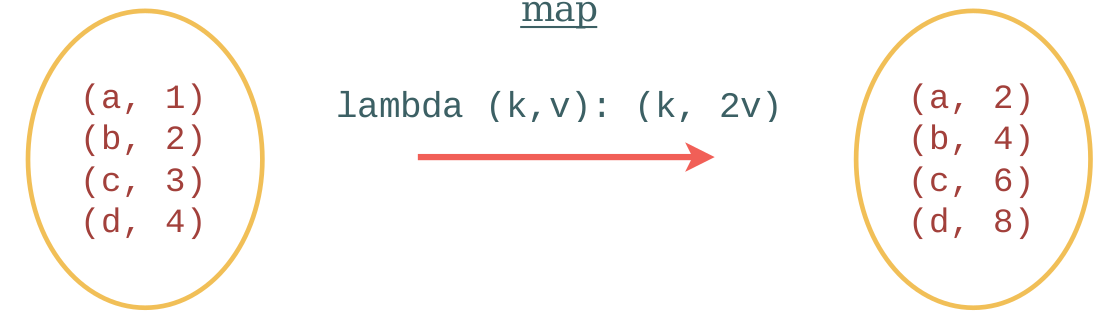
\includegraphics{fig/map-example.png}

    \+
    \texttt{rdd2 = rdd1.map(F)}
\end{center}
\end{frame}


\begin{frame}
  \frametitle{\texttt{flatMap} transformation}

  \begin{center}
    Apply a (possibly one-to-many) function~$F$
    to each element of a given RDD.  Expect that $F$ produces a list for each
    element of the input RDD, and make a new (output) RDD from the concatenation
    of such lists.

    \+
    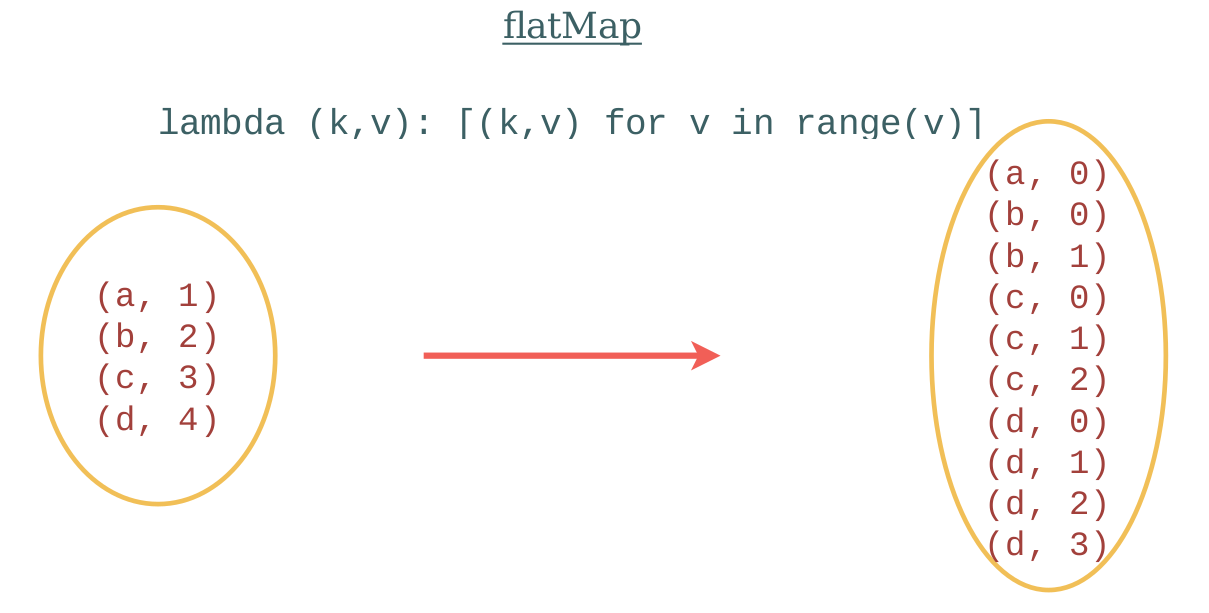
\includegraphics[scale=0.8]{fig/flatMap-example.png}

    \texttt{rdd2 = rdd1.flatMap(F)}
\end{center}
\end{frame}


\begin{frame}
  \frametitle{\texttt{filter} transformation}

  \begin{center}
    Create a new RDD by selecting elements from the input RDD on which
    function~$F$ takes a ``true'' value.

    \+
    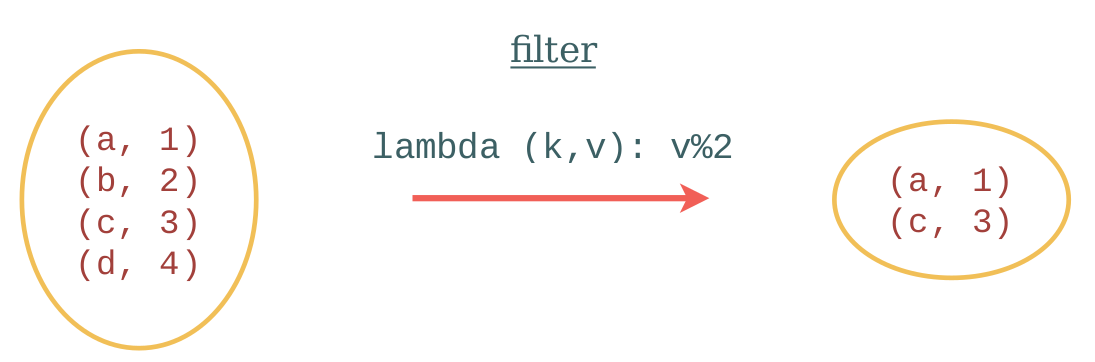
\includegraphics{fig/filter-example.png}

    \+
    \texttt{rdd2 = rdd1.filter(F)}
\end{center}
\end{frame}


\begin{frame}
  \frametitle{\texttt{reduceByKey} transformation}

  \begin{center}
    Group elements by key and reduce the resulting sequence of values to form a
    new RDD.

    \+
    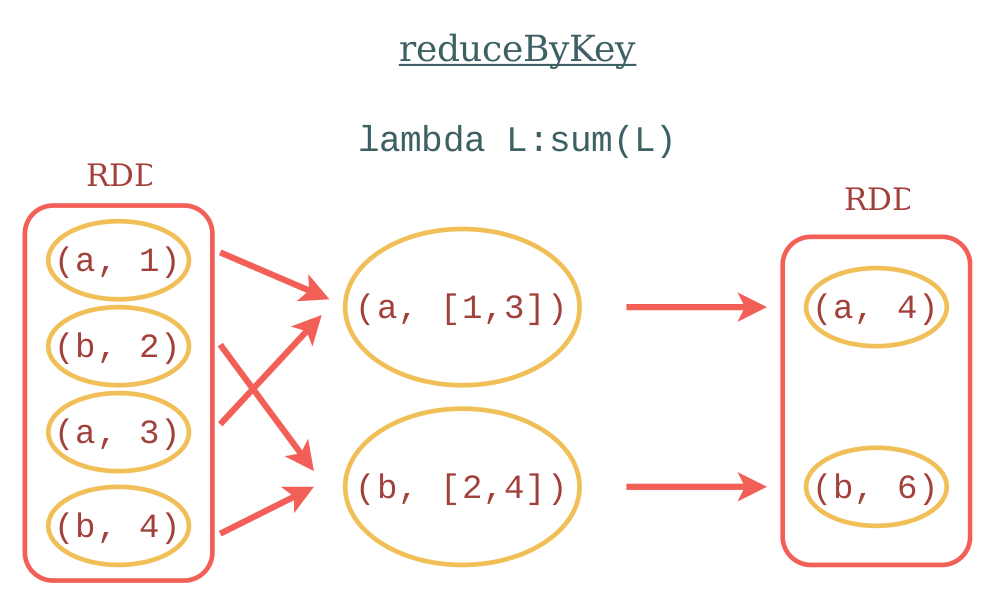
\includegraphics{fig/reduceByKey-example.png}
  \end{center}
\end{frame}


\begin{frame}[fragile]
  \frametitle{Other transformations on Key/Value RDDs}

  Other transformations include:
  \begin{itemize}
  \item \lstinline|rdd2 = rdd1.groupBy(f)| \\
    Create a key/value RDD \texttt{rdd2} using function \texttt{f} to
    compute the key corresponding to each value in \texttt{rdd1}.
  \item \lstinline|rdd2 = rdd1.keys()| \\
   \lstinline|rdd2 = rdd1.values()| \\
    \texttt{rdd2} is the set of keys or values of \texttt{rdd1}
  \item \lstinline|rdd2 = rdd1.mapValues(f)| \\
    Pass each value in \texttt{rdd1} through function \texttt{f}
    without changing the keys.
  \item \lstinline|rdd1 = rdd2.zip(rdd3)| \\
    \texttt{rdd1} is the RDD of pairs whose first element comes from
    \texttt{rdd2} and second element from \texttt{rdd3}
\end{itemize}
\end{frame}


\begin{frame}[fragile]
  \frametitle{Set-theoretic transformations}

  Other transformations include:
  \begin{itemize}
  \item \lstinline|rdd3 = rdd1.cartesian(rdd2)| \\
    \texttt{rdd3} is the set of pairs \texttt{(a, b)} where \texttt{a}
    is an element of \texttt{rdd1} an \texttt{b} is an element of
    \texttt{rdd2}
  \item \lstinline|rdd3 = rdd1.intersection(rdd2)| \\
   \lstinline|rdd3 = rdd1.subtract(rdd2)| \\
   \lstinline|rdd3 = rdd1.union(rdd2)| \\
    \texttt{rdd3} is the set-theoretic intersection/difference/union of \texttt{rdd1} and \texttt{rdd2}
\end{itemize}
\end{frame}


\begin{frame}[fragile]
  \frametitle{Other transformations}

  Other transformations include:
  \begin{itemize}
  \item \lstinline!rdd2 = rdd1.distinct()! \\
    only retain the unique elements of the entire RDD
  \item \lstinline|rdd2, rdd3 = rdd1.randomSplit([w1, w2])| \\
    Split \texttt{rdd1} into \texttt{rdd2}, \texttt{rdd3} by randomly
    assigning elements with probabilities \texttt{w1}, \texttt{w2}.
  \item \lstinline!rdd2 = rdd1.sortBy(f)! \\
    \texttt{rdd2} has the same elements as \texttt{rdd1}, sorted so
    that \texttt{f} takes ascending values.
\end{itemize}
\end{frame}


\begin{frame}
  \frametitle{Lineage}

  \textbf{Transformations are evaluated ``lazily'': only executed once an
    \emph{action} is performed.}

  \begin{itemize}
  \item
    When an RDD is transformed, this \textbf{transformation} is not
    automatically carried out.
  \item
    Instead, the system remembers how to get from one RDD to another and
    only executes whatever is needed for the \textbf{action} that is being
    done.
  \item
    This allows one to build up a complex ``pipeline'' and easily
    tweak/rerun it in its entirety.
  \end{itemize}
\end{frame}


\begin{frame}
  \small

  \begin{exercise*}[2.D]
    Implement a the ``word count'' algorithm using PySpark, and use it
    to count the words in file \texttt{hdfs:///shakespeare.txt.gz}

    \+
    What are the 5 most frequent words?

    \+ \smaller
    \emph{Hint:} The ``word count'' algorithm is comprised of the
    following steps:
    \begin{itemize}
    \item Read lines of a text file into an RDD;
    \item Transform the RDD by splitting each line at blank spaces;
    \item Create a key/value RDD by pairing each word with the value \texttt{1};
    \item Sum the values associated with each word.
    \end{itemize}

  \end{exercise*}

  \+
  \begin{exercise*}[2.E]
    Write a solution to Exercise~1.E using PySpark.
  \end{exercise*}
\end{frame}


\begin{frame}[fragile]
  \frametitle{Recap of RDD usage}
  \begin{enumerate}
  \item Create a \texttt{SparkSession} object.\footnote{%
      \smaller
      In Spark 1.x this was called \texttt{SparkContext}.
    }%
  \item Inject data into Spark:
    \lstinline|rdd = sc.parallelize(data)|
  \item Build a computation DAG by chaining \emph{transformations}:
    \begin{python}
step1 = rdd.flatMap(lambda line:
            [(w,1) for w in line.split()])
step2 = step1.reduceByKey(lambda a,b: a+b)
    \end{python}
  \item Extract final data with \emph{actions}:
    \lstinline|wc = step2.collectAsMap()|
  \end{enumerate}
\end{frame}


\end{document}

%%% Local Variables:
%%% mode: latex
%%% TeX-master: t
%%% End:
